\documentclass[tikz,border=3pt]{standalone}
\usetikzlibrary{arrows.meta,decorations.pathmorphing}
\begin{document}
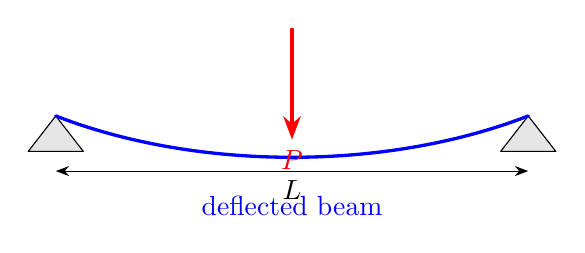
\begin{tikzpicture}[x=1cm,y=1cm,>=Stealth,line cap=round,line join=round]
  \draw[fill=gray!20] (-.35,0) -- (.35,0) -- (0,.45) -- cycle;
  \draw[fill=gray!20] (5.65,0) -- (6.35,0) -- (6,.45) -- cycle;
  \draw[blue,very thick,decorate,
    decoration={bent,aspect=.3,amplitude=-7mm}]
    (0,.45) -- (6,.45);
  \draw[->,red,very thick] (3,1.55) -- (3,.15) node[below] {$P$};
  \draw[<->,thin] (0,-.25) -- (6,-.25) node[midway,below] {$L$};
  \node[blue,below] at (3,-.45) {deflected beam};
\end{tikzpicture}
\end{document}
